\chapter{Алгоритмы}
Поскольку WWW представляет собой крайне сложную среду, которая постоянно развивается, предпочтение было отдано практическому подходу:
\begin{enumerate}
 \item запустить систему без модификаций;
 \item найти самое слабое место в системе;
 \item принять меры по его устранению;
 \item перейти к пункту \textit{2}.
\end{enumerate}
\section{Ранжирование}
При работе системы в стандартной конфигурации было замечено, что только из 10\% скачиваемых веб-страниц выделяются документы. Это происходит из-за неоптимального упорядочивания ссылок из \textit{сrawldb}.

Определение порядка выбора URL для скачивания существенно сказывается на эффективности работы робота.\cite{crawl}\cite{focused}\cite{opic} Порядок неважен только в том случае, если робот нацелен на одноразовое скачивание всего Web, и нагрузка создаваемеая роботом на целевые сайты не важна, так как тогда каждая известная URL будет в конце концов загружена. Однако большинство роботов не способно посетить каждый URL по трем основным причинам:
\begin{itemize}
 \item Ограничение по ресурсам --- размер хранилища, ширина канала, CPU time для обработки страниц.
 \item Сбор документов занимает время, поэтому в определенный момент робот вынужден заново посещать некоторые страницы для нахождения изменений.
 \item Динамическое создание страниц --- сейчас большинство сайтов разадают не статический контент, а создают его динамически при помощи скриптов обрабатывающих URL и возвращающих результат, таким образом количество страниц на сайте может быть неограничено.
\end{itemize}

Во всех остальных случаях существенно что бы робот сначала посещал ``важные'' страницы. Ранжирование отвечает за определенеие того, на сколько URL ``важна''.
В Nutch порядок выбора URL определяется в плагинах подключенных к точке расширения \textit{ScoringFilter}, в результате работы которых каждой URL сопоставляется \textit{score}. На каждой итерации для скачивания выбираются URL с наибольшим score.

В стандартной конфигурации Nutch для выбора ссылок используется \textit{OPIC Score} плагин.
\subsection{OPIC}
\textit{OPIC} --- On-Line Page Importance Computation\cite{opic}. Данный алгоритм расчитывает важность страницы на основе важности страниц на него ссылающихся. В отличии от off-line методов, когда сначала скачивается часть Web, а потом на основе полученного графа ссылок вычисляется важность страниц, этот метод позволяет работать когда большая часть сетевого графа еще не известна.

В Nutch реализована упрощенная версия данного алгоритма, при котором в момент скачивания страницы к score каждой из ссылок с нее (\textit{outlink}) добавляется $S_{0}/n$ где $S_{0}$ --- $score$ скачанной страницы, а $n$ --- число исходящих ссылок. Данный способ плохо подходит для поиска новостей, поскольку для новостей основным признаком ``важности'' веб-страницы является присутствие в нем текста новости, что на практике не связано с количеством входящих ссылок.

Поскольку в системе идентификация новостей производится только по URL возникает желание скачивать только те URL, которые подходят под правла.

\subsection{Предложенный алгоритм}
Так как в Nutch можно использовать одновременно сразу несколько ScoringFilter'ов (полученные из различных алгоритмов \textit{score} просто перемножаются), вместо изменения стандартного метода следует создать отдельный плагин, который всем новым поступающим в систему URL которые подходят под правила разбора устанавливать $score=s_{fit}$ и $s_{n}$ для остальных.
\subsection{Особенности реализации}
Данная функциональность была реализована при помощи двух плагинов. Первый проверяет является ли URL ``полезной'', и добавляет необходимую информацию в $crawldatum$ (в \textit{crawldb} хранятся записи вида $\langle URL, crawldatum\rangle$, где \textit{crawldatum} --- различная дополнительная информация об URL), а второй выставляет ранг согласно $crawldatum$ и настроек приложения. Такое разбиение было сделано потому что информация о том, что url является ``полезной'', представляет собой интерес и без использования данного ранжирования (например, это было использовано при получении статистики).
\subsubsection*{SkaiScoringMeta}
\label{sec:scoringmeta}
SkaiScoringMeta --- плагин являющийся расширением к точке ScoringFilter, выделяющий ``полезные'' URL. Для хранения дополнительной информации в $crawldatum$ используется поле $metaData$, которое представляет собой набор пар вида $\langle key, value\rangle$
Для сохранения индикатора ``полезности'' в мета данные $crawldatum$ добавляется пара $\langle skai.scoring.fit, true\rangle$.

Для определения ``полезности'' URL используется кэш с регулярными выражениями, загружаемыми из базы данных при инициализации. Поскольку таких регулярных выражений может быть много (хотя бы по одному на сайт) и они разбиты по доменам, для сокращения времени проверки каждой URL используется хэш вида $\langle domainname, regex^{+}\rangle$, таким образом время проверки URL практически не зависит от числа доменов.

Так же, для уменьшения числа проверок, метаданные добавляются не в момент первого обнаружения ссылки системой (сразу после разбора веб-страницы), а только в момент добавления уникальной URL в \textit{crawldb}, что уменьшает число проверок приблизительно в 10 раз, так как в среднем только 9\% исходящих со страницы ссылок не были ранее известны.
\subsubsection*{SkaiScoring}
SkaiScoring --- плагин являющийся расширением к точке ScoringFilter, выставляющий $score$. Для ссылок только что попавших в систему, зависимости от наличия мета тега, выставляет значения $score$ либо $s_{fit}$, либо $s_{n}$, где коэффициенты $s_{fit}$ и $s_{n}$ получаются из файла конфигурации Nutch.
\subsection{Результат}
При использовании стандартных ScoringFilter'ов в среднем за цикл, из всех скачиваемых ссылок ``полезных'' скачивалось порядка 10\% (В качестве пространства поиска использовалось 40 крупнейших СМИ, на каждой итерации выбиралось 20000 ссылок, ``полезными'' признавались непосредственно новости). А при использовании данных плагинов уже на ранней стадии сборки порядка 80\% ссылок были ``полезными'' (Рис.~\ref{ris:score}). Благодаря предложенным оптимизациям время цикла практически не изменилось по сравнению с временем работы в стандартной конфигурации. Таким образом было получено увеличение эффективности в восемь раз по сравнению с базовой реализацией Nutch.

\begin{figure}[h!]
 \center{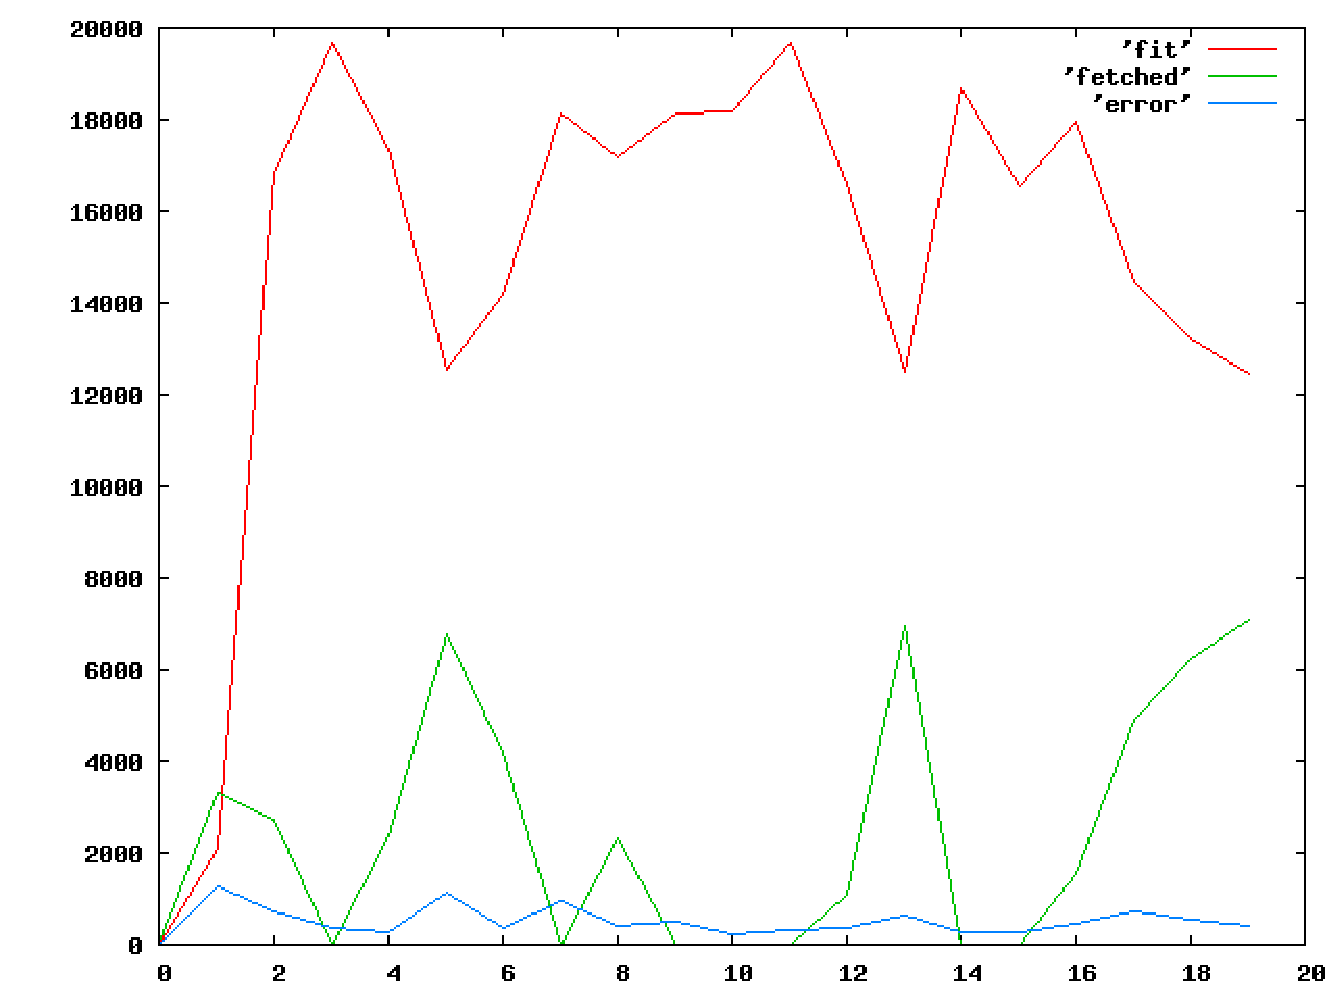
\includegraphics[width=0.8\linewidth]{img/scoring}}
 \caption{График зависимости числа ссылок от номера итерации. fit---число полезных ссылок, fetched---число скачанных ссылок не являющихся полезными, error---число ошибок при скачивании}
 \label{ris:score}
\end{figure}

\section{Работа Nutch с индексом}
Время используемое для слияния полученного из сегмента индекса с основным растет пропорционально размеру индекса. Этот этап не работает через MapReduce и фактически выполняется на одной машине, что приводит к простою кластера. Для индекса содержащего 2 миллиона документов (70GB) только копирование индекса из HDFS в локальную файловую систему и обратно занимает больше двух часов (при скорости локальной сети 20Mb/s), а общее время работы достигает 11 часов ($2\times2,5$ GHz 2007 Xeon, 1,7GB RAM, скорость последовательного доступа к диску 50MB/s). При размере \textit{crawldb} в 80 миллионов ссылок и генерации сегмента в 80 тысяч URL на слияние индека уходит 68\% от общего времени цикла (на кластере из трех узлов).
\subsection{Lucene}
\textit{Lucene} --- библиотека полнотекстовго поиска. Индекс Lucene построен по принципу обратного файла (инвертированного индекса). Сам индекс состоит из сегметнов, каждый из которых грубо говоря представляет отсортированный список термов. Для ускорения поиска сегменты ``склеиваются'' в один. Операция ``склеивания'' представляет собой этап слияния из сортировки слиянием, и производится за время прямопропорциональное сумме размеров склеиваемых сегментов. По-умолчанию Nutch хранит индекс в одном сегменте, к которому на каждой итерации ``приклеиваются'' новые сегменты индекса, таким образом за каждую итерацию весь индекс перезаписывается.

Было рассмотрено несколько подходов к решению данной проблемы:
\begin{itemize}
 \item \textbf{Асинхронное обновление} --- выделяется отдельный поток, который  находит все новые сегменты, скачивает их и независимо от процесса основной сборки и обновляет индекс. При этом время на слияние индексов не влияет на скорость скачивания документов, однако, уже при размере индекса в 5,3 миллионов документов индекс будет обновляться только один раз за сутки, из-за чего новости за последние 30 часов никогда не появятся в индексе (время на слияние+время цикла).
 \item \textbf{Изменение политики слияния} --- хранение индекса в одном сегменте требует перезаписи всего инедса при каждом обновлении. При этом если вообще не ``склеивать'' сегменты, существенно падает время поиска в индексе, поскольку приходится искать терм в большом числе словарей. Необходимо разработать алгоритм который позволял бы контролировать число сегментов, при этом не перезаписывая основную часть индекса.

Приблизительно, время выполнения запроса можно оценить следующим образом: $t_{q} = \sum\limits_{s\in S} td_{s} + ti$, где $td_{s}$ это поиск термов в словаре сегмента $s$, а $ti$ --- время на пересечение списков документов соответствующих термам. Причем $ti$ прямопропорционально количеству документов соответсвующих термам, а $td_{s} = O(\log n_{s})$, где $n_{s}$ --- размер словаря сегмента, который практически не зависит от размера сегмента, и можно считать константой. Само время ``склеивания'' сегментов прямопропорционально их размеру, из чего следует что эффективнее всего склеивать между собой самые маленькие сегменты. 
 
\end{itemize}
\subsection{Алгоритмы}
\subsubsection{Асинхронное обновление}
Поскольку появление новых сегментов происходит один раз за несколько часов, было решено создать процесс, который через определенные промежутки времени проверяет наличие новых сегментов и скачивает их стандартными средствами Hadoop в локальную файловую систему клента работающего с индексом, после чего сообщает клиенту о необходимости подключить новые сегменты.
\subsubsection{Политика слияния}
Индексам присваивается некий уровень $l$, так же известно максимальное количество сегментов на каждом уровне $N_{l}$. Всем только что скачанным сегментам присваивается $l=0$, в тот момент когда количество индексов на каком-то из уровней превышает $N_{l}$ они ``склеиваются'' в один сегмент уровня $l+1$.
\subsection{Особенности реализации}
\subsubsection{Асинхронное обновление}
Как только заканчивается индексация нового сегмента, к имени сегмента добавляется префикс \textit{ready}. Процесс просматривает папку с сегментами в HDFS и при наличии сегментов с такими префисками скачивает их и убирает префикс, после чего сообщает клиенту HTTP запросом о необходимости подключить новый сегмент. При таком подходе аварийное завершение процесса обновления не влечет никаких последсвий --- достаточно просто заново его запустить, и отключение основного цикла сборки никак не сказывается на процесс обновления (кроме того, что не появляется новых сегментов индекса).
\subsubsection{Политика слияния}
Индексы были разбиты на следующие уровни:
\begin{enumerate}
 \item new --- новые сегменты;
 \item daily --- сегменты за день;
 \item weeky --- сегменты за неделю;
 \item monthly --- сегменты за 4 недели;
 \item 1-level --- сегменты за 4 месяца ($4\times4$ недели);
 \item k-level --- сегменты получаемые при слиянии четырех k-1-level.
\end{enumerate}
В конце каждого дня все новые индексы объединяются в дневные, как только их набирается 7 --- они склеиваются в недельные и.т.д. Сама функциональность была реализована как \textit{Groovy} скрипт.
\subsection{Результат}
Благодаря асинхронному обновлению время цикла уменьшилось на 68\%, однако возрасла нагрузка на сервер осуществляющим поиск, так как слияние индексов стало происходить на нем, однако, за счет новой политики слияния, каждый документ в индексе перезаписывается не более 5 раз за год, что дает в сумме не более 80 часов в год при конечном индексе в 10 миллионов документов.
 
